
\section{Introduction}
\begin{wrapfigure}{r}{0.45\textwidth}
%\vspace{-20pt}
\vspace{-35pt}
\centering
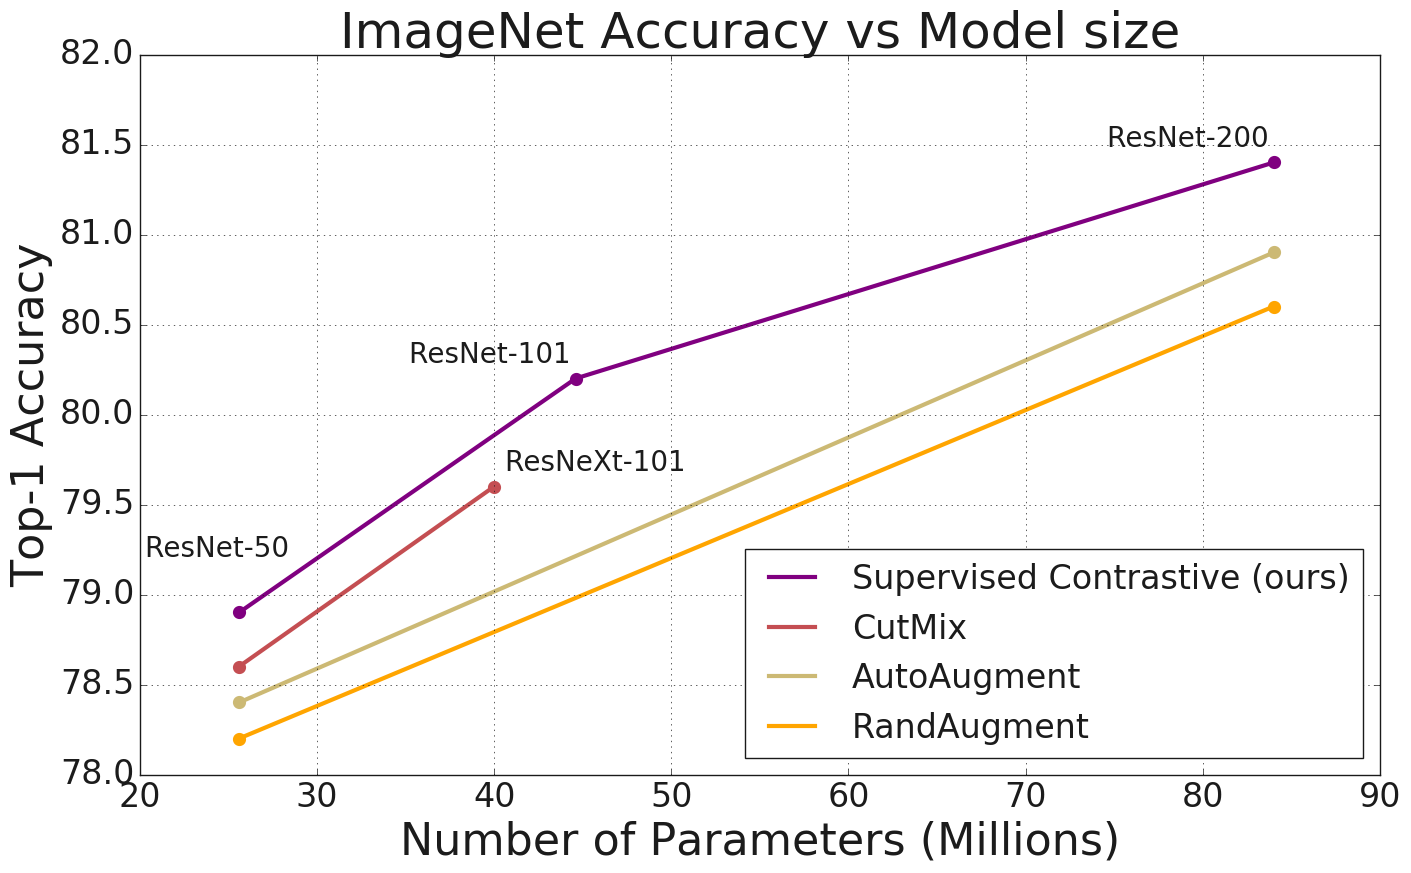
\includegraphics[width=\linewidth]{./figs/teaser_fig2}
{\caption{\small Our SupCon loss consistently outperforms cross-entropy with standard data augmentations. We show top-1 accuracy for the ImageNet dataset, on ResNet-50, ResNet-101 and ResNet-200, and compare against AutoAugment \cite{cubuk2019autoaugment}, RandAugment \cite{cubuk2019randaugment} and CutMix \cite{yun2019cutmix}. 
}
\label{fig:imagenet_top1_teaser} }
%\vspace{-40pt}
\vspace{-47pt}
\end{wrapfigure}

\begin{figure*}[t!]  
 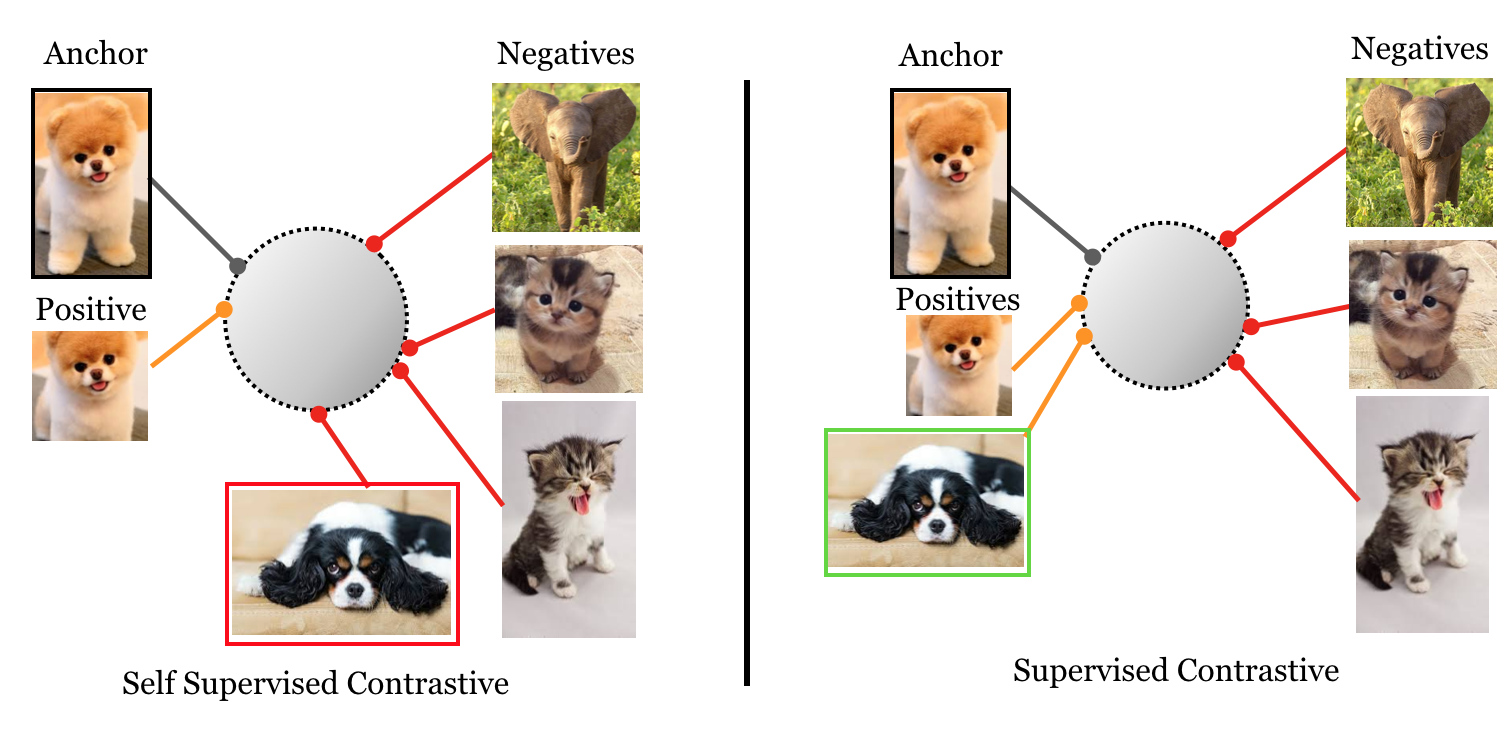
\includegraphics[width=\linewidth]{./figs/teaser_fig_new1}
 {\caption{\small Supervised vs. self-supervised contrastive losses: The self-supervised contrastive loss (left, Eq. \ref{eqn:self_loss}) contrasts a \emph{single} positive for each anchor (i.e., an augmented version of the same image) against a set of negatives consisting of the entire remainder of the batch. The supervised contrastive loss (right) considered in this paper (Eq. \ref{eqn:supervised_loss}), however, contrasts the set of \emph{all} samples from the same class as positives against the negatives from the remainder of the batch. As demonstrated by the photo of the black and white puppy, taking class label information into account results in an embedding space where elements of the same class are more closely aligned than in the self-supervised case.}  
 \label{fig:teaser1}
}
 \vspace{-20pt}
\end{figure*}

The cross-entropy loss is the most widely used loss function for supervised learning of deep classification models. A number of works have explored shortcomings of this loss, such as lack of robustness to noisy labels \cite{zhang2018generalized,sukhbaatar2014training} and the possibility of poor margins \cite{elsayed2018large,liu2016large}, leading to reduced generalization performance. However, in practice, most proposed alternatives have not worked better for large-scale datasets, such as ImageNet \cite{deng2009imagenet}, as evidenced by the continued use of cross-entropy to achieve state of the art results \cite{cubuk2019autoaugment,cubuk2019randaugment,xie2019self,kolesnikov2019large}. 


In recent years, a resurgence of work in contrastive learning has led to major advances in self-supervised representation learning \cite{wu2018unsupervised,henaff2019data,oord2018representation,tian2019contrastive,hjelm2018learning,chen2020simple,he2019momentum}. The common idea in these works is the following: pull together an anchor and a ``positive" sample in embedding space, and push apart the anchor from many ``negative" samples. Since no labels are available, a positive pair often consists of data augmentations of the sample, and negative pairs are formed by the anchor and randomly chosen samples from the minibatch. This is depicted in Fig. \ref{fig:teaser1} (left). In \cite{oord2018representation,tian2019contrastive}, connections are made of the contrastive loss to maximization of mutual information between different views of the data.

In this work, we propose a loss for supervised learning that builds on the contrastive self-supervised literature by leveraging label information.
Normalized embeddings from the \emph{same class} are pulled closer together than embeddings from \emph{different classes}. Our technical novelty in this work is to consider \emph{many positives} per anchor in addition to many negatives (as opposed to self-supervised contrastive learning which uses only a single positive). These positives are drawn from samples of the same class as the anchor, rather than being data augmentations of the anchor, as done in self-supervised learning. While this is a simple extension to the self-supervised setup, it is non-obvious how to setup the loss function correctly, and we analyze two alternatives. Fig.~\ref{fig:teaser1} (right) and Fig.~1 (Supplementary) provide a visual explanation of our proposed loss. Our loss can be seen as a generalization of both the triplet \cite{weinberger2009distance} and N-pair losses \cite{sohn2016improved}; the former uses only one positive and one negative sample per anchor, and the latter uses one positive and many negatives. The use of many positives and many negatives for each anchor allows us to achieve state of the art performance without the need for hard negative mining, which can be difficult to tune properly. To the best of our knowledge, this is the first contrastive loss to consistently perform better than cross-entropy on large-scale classification problems. Furthermore, it provides a unifying loss function that can be used for either self-supervised or supervised learning.


Our resulting loss, SupCon, is simple to implement and stable to train, as our empirical results show. It achieves excellent top-1 accuracy on the ImageNet dataset on the ResNet-50 and ResNet-200 architectures \cite{he2016deep}. On ResNet-200 \cite{cubuk2019autoaugment}, we achieve a top-1 accuracy of $81.4\%$, which is a $0.8\%$ improvement over the state of the art \cite{lim2019fast} cross-entropy loss on the same architecture (see Fig. \ref{fig:imagenet_top1_teaser}). The gain in top-1 accuracy is accompanied by increased robustness as measured on the ImageNet-C dataset \cite{hendrycks2019benchmarking}. Our main contributions are summarized below:

\begin{enumerate}[leftmargin=*,topsep=0pt,itemsep=-1ex,partopsep=1ex,parsep=1ex]
    \item We propose a novel extension to the contrastive loss function that allows for multiple positives per anchor, thus adapting contrastive learning to the fully supervised setting. Analytically and empirically, we show that a na{\"i}ve extension performs much worse than our proposed version.
    \item We show that our loss provides consistent boosts in top-1 accuracy for a number of datasets. It is also more robust to natural corruptions.
    \item We demonstrate analytically that the gradient of our loss function encourages learning from hard positives and hard negatives. %
    \item We show empirically that our loss is less sensitive than cross-entropy to a range of hyperparameters. %
\end{enumerate}
\vspace{-10pt}

\if{false}
Self-supervised learning is a branch of unsupervised learning that relies on natural supervision cues, usually exploiting structure in data. Examples include co-occurring modalities \cite{sun2019videobert,arandjelovic2017look,tian2019contrastive}, spatio-temporal structure \cite{henaff2019data,devlin2018bert} or generated structure \cite{hjelm2018learning}. The structure provides a form of weak supervision which can be exploited to learn powerful embeddings.  The resulting embeddings can be used for downstream tasks such as classification or object detection. Self-supervised learning has seen significant strides in recent years in multiple domains such as images, videos and natural language. 

The basic form of the loss function is inspired by noise contrastive estimation \cite{gutmann2010noise} and N-pair losses \cite{sohn2016improved}, which allows learning of unnormalized statistical models by training a binary classifier to distinguish between samples from noise and data distributions. In contrastive learning as used in the current paper and related work, we also employ a classification like approach. However, here the idea is to increase the similarity between positive pairs of samples and decrease similarity between negative pairs. Similarity is usually defined as the inner product between low-dimensional embeddings. The resulting embeddings are then shown to be a very good representation by being trained on various downstream transfer tasks. 

In addition to excellent empirical performance, theoretical motivation for unsupervised contrastive learning has been provided by \cite{arora2019theoretical}, where it is shown that the contrastive loss is an upper bound on downstream supervised loss, under the assumption that the data distribution is stationary between pre-training and downstream stages. Furthermore \cite{arora2019theoretical} suggest a novel loss that incorporates multiple positive samples, compared to the usual loss that contrasts a single positive with many negatives. The use of multiple positives provides a tighter bound on the downstream supervised loss. Our new loss function is closely related to this idea.

The family of \emph{metric losses} are intimately related to the contrastive loss. The canonical example is the triplet loss function  \cite{weinberger2009distance}, which introduced the idea of decreasing the embedding distance between positive pairs of samples, and push apart negative pairs. The triplet loss has proven very powerful in learning high performing embeddings e.g. \cite{schroff2015facenet,chopra2005learning}, and has often been used when the total number of categories are unknown, but it is known whether or not two samples are of the same category. The contrastive loss as used in this paper is very similar to the metric loss when we use a single positive and negative example for each anchor sample. However, the use of larger numbers of positives and negatives are very important for performance.

\fi